\documentclass[11pt]{article}

\usepackage[margin=1in]{geometry}
\usepackage{amsmath, amssymb, amsthm, mathtools}
\usepackage{fancyhdr}
\usepackage{hyperref}
\usepackage{tikz}
\usepackage{graphicx}
% \begin{figure}[htbp] % [htbp] 告诉 LaTeX 尽量放在这里、顶部、底部或单独一页
%     \centering % 图片居中
%     
\includegraphics[width=0.5\linewidth]{HW3/笔记 2025年11月2日.jpeg} 
%     \caption{这是 MATH154 HW1 的图示} % 图片下方的标题
%     \label{fig:graph1} % 用于文中引用，比如 "如图 \ref{fig:graph1} 所示"
% \end{figure}

\setlength{\parindent}{0pt}
\setlength{\parskip}{0.5em}

\newcommand{\R}{\mathbb{R}}
\newcommand{\N}{\mathbb{N}}
\newcommand{\Z}{\mathbb{Z}}
\newcommand{\Q}{\mathbb{Q}}
\newcommand{\C}{\mathbb{C}}

\newenvironment{problem}[1]
  {\section*{Problem #1}}
  {}



\begin{document}

\title{Homework 1}
\author{Jamie Meng}
\date{\today}

\maketitle
\section{Problem 1}
\subsection*{(a)}
Because we delete a leaf, which is a vertex, so the graph will have one less vertices, so the number of vertices is $v(T)-1$.

Because we deleted one vertex without adding any edges or vertices, we did not add circles to the graph, and new graph is acyclic. Also, the leaf has only degree 1, so there is one edge connected to it, and itself is deleted. Therefore, the grahp is still connected.

Therefore, deleting a leaf from a tree T with $v(T ) \ge2 $produces a tree with $v(T ) - 1$ vertices.

\subsection*{(b)}
We can prove by indcution:

Basecase: if there are 2 vertices and we delete one vertex from them. Becasue they both have degree of one. And delete them leave one vertex left, so the component number is 1. Therefore, the statement is true for base case.

Induction hypothesis:
Deleting a vertex v from a tree T with$ v(T )=n-1$ produces a forest with $d_T (v) $components.

If we have a tree T with n vertices, we can delete one leaf(every tree has at least one leaf) to make it a n-1 vertices tree T'. Then deleting a vertex v from a tree T' produces a forest with $d_{T'} (v) $components. Then, if we need to delete one vertex from T, if we do not delete the leaf and the neighbor of that leaf. Then, the leaf must connected to a componet when we delete the same vertex in V', whihc won't add more components. Therefore, deleting a vertex v(not the leaf and its neighbor) from a tree T produces a forest with $d_T (v)$components

If we delete the leaf's neighbor n: in T' if we delete it, it will produces a forest with $d_{T'} (n)$. In T, all components produced in T' will also be produced. And leaf itself will be a component, so in total it will produced $d_{T'} (n)+1$components. Becasue it degree become$ d_{T'} (n)+1$ after add the leaf back, the statement is still true.

If we delete the leaf, the rest of the tree is still a component, so there is still one component. Becasue leaf's degree is one, the statement is still true.

Inconclusion, deleting a vertex v from a tree T produces a forest with $d_T (v)$components.

\subsection*{(c)}
Basecase: if there is one vertes, then itself is a path.

Induction hypothesis: for any tree T with n-1 vertices the following is true: if $\Delta(T ) \le 2$,then T is a path.

If we have a tree T with n vertices and $\Delta(T ) \le 2$, then we can delete a leaf to make a tree with n vertices, and it is path. Then we add back the leaf. Because $\Delta(T ) \le 2$, we can only add it in the end of the path, otherwise, it will add one to the degree of middle vertices in the path, making it degree become 3. When we add a vertex to the end of a path, the path extends one vertex and is still a path. Therefore, for any tree T if $\Delta(T ) \le 2$,then T is a path.

\subsection*{(d)}
Method 1:
Look at the vertex v with $\Delta(T)$ degrees. 

For each of its neighbors $n_i$, do the following:

Consider the longest path start from v, then to $n_i$. There exists the end point of the path. And the end point is a leaf $l_i$. Becasue if it has degree 2, the other neighbor cannot connect to any vertices already on the path, since otherwise there will be a cycle. Therefore, the path can extend making it not the longest path, which is a contradition.

These produced $l_i$ can not be duplicate. Because if they are same such as $l_1$ and $l_2$, then there exist a path from $l_1$ to $n_1$ and a path $l_2$ to $n_2$, so there is a cycle: $l_1$-$n_1$-v-$n_2$-$l_1$, making the original tree not a tree, which is a contradition.

Therefore, there are at least $\Delta(T)$ leaves, because there are $\Delta(T)$ $l_i$.


Method 2: Induction:

Basecase: For a 2 vertices tree. There are 2 leaves and $\Delta(T)=1$, so the statement is true.

Induction hypothesis:tree T with n-1 vertices contains at least $\Delta(T) $ leaves.

For a tree with n vertices, there must be a leaf. Then we delete it to make a tree T'.
T' has at least $\Delta(T') $ leaves. 
Then, we add back the leaf, if the leaf connects to the vertices with most neighbors. Then, $\Delta(T) =\Delta(T')+1$. And T also have one more leaf. So the statement is still true.

If it does not connect to vertices with most neighbors, then $\Delta(T) =\Delta(T')$. Because we add a leaf to it, the number of leaves will add one if the leaf's neighbor is not a leaf originally. The number of leaves may also unchanged, if the leaf's neighbor is a leaf, and we add a new leaf while make its neighbor not a leaf, the number of leaves is unchanged. But, anyway, the number of leaves won't decrease, so the statement is still true.

Therefore, tree T contains at least $\Delta(T) $ leaves.

\section{Problem 2}
\subsection*{(a)}
See the graph above.
\begin{figure}[h] % [htbp] 告诉 LaTeX 尽量放在这里、顶部、底部或单独一页
    \centering % 图片居中
    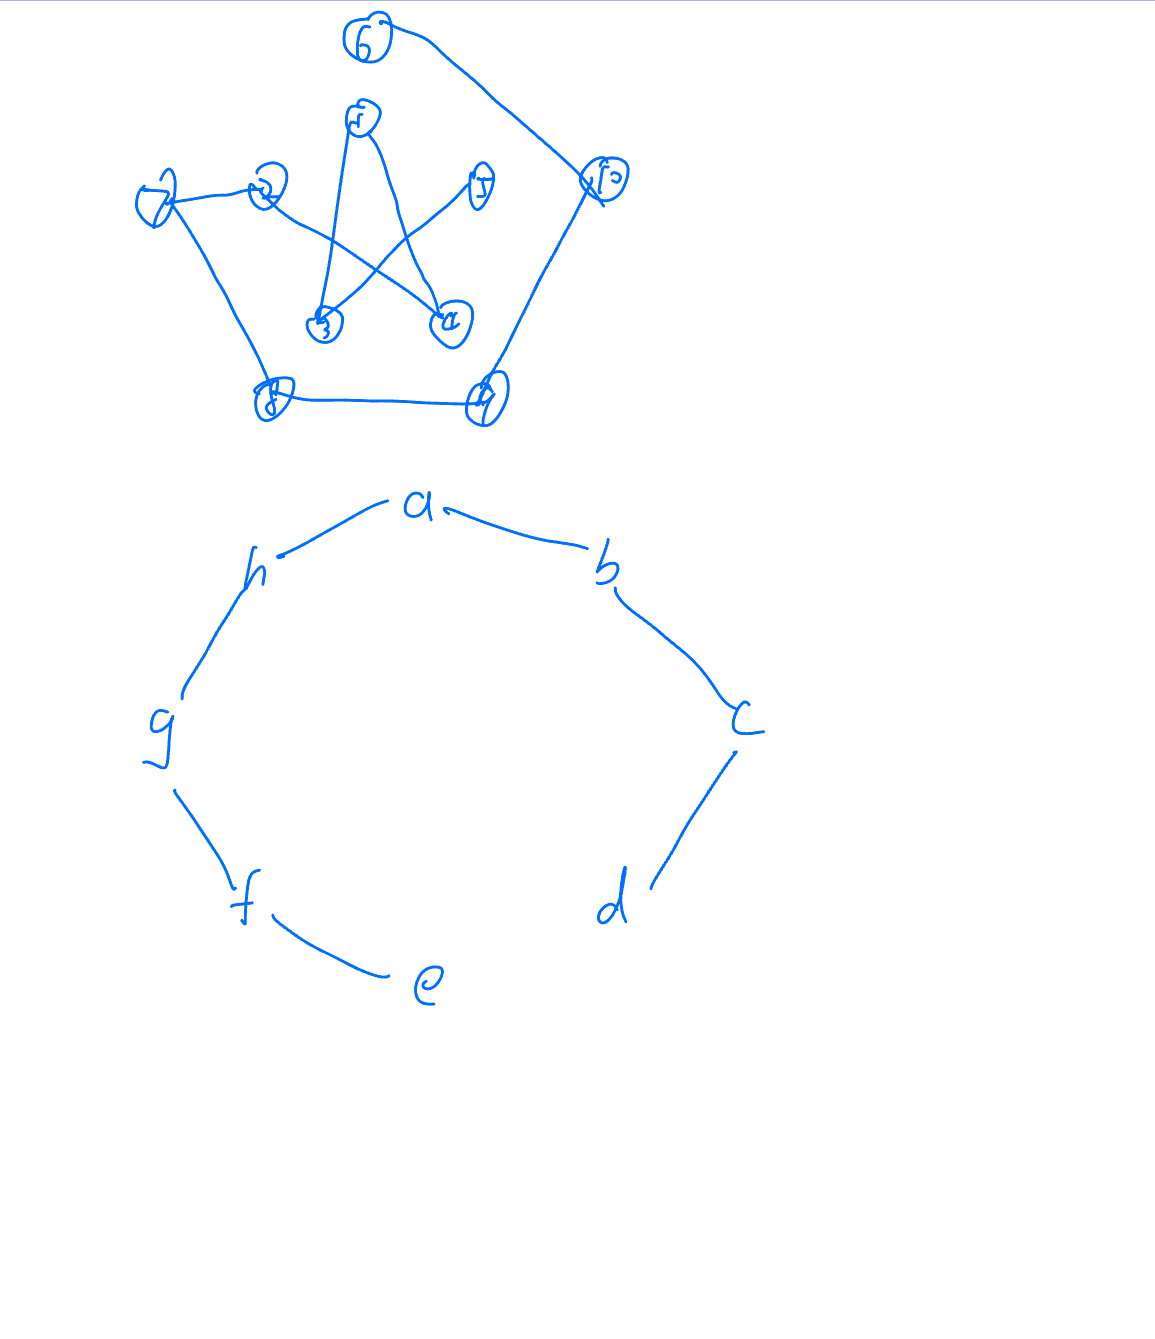
\includegraphics[width=0.5\linewidth]{笔记 2025年11月2日.jpeg} 
    \caption{Problem 2 (a)}
\end{figure}

\subsection*{(b)}
When we get the graph G, we can remove some edges that is a part of some cycle to make it become a forest. Let's see how many edges we need to remove. 

The number of edges of a forest is $v(G)-n$, n is the number if component which > 0.

So the number of edge we need to remove is  $e(G)-v(G)+n$, which is at least $e(G)-v(G)+1$.

Each time we remove a edge, the number of cycle will at lesat decrease 1. Therefore, we removed at least $e(G)-v(G)+1$ cycles. Therefore, any graph G contains at least $e(G)-v(G)+1$ many cycles.

\subsection*{(c)}
Prove for $\Rightarrow $

Proof by contradiction:
If some spanning tree do not contain the cuting edge. Then this edge is removed. The order of removing the edges does not matter, so we can remove it first and the graph become not connected. When we are romove other edges, the graph remains uncnonected, because no edges are added. Therefore, the final graph is not connected and it cannot be tree, which is a contradition. Therefore, no spanning tree contain the cutting edge.

Prove for $\Leftarrow $

Prove its contrapositive, that is if a edge is not a cutting edge, then it's not in every spanning tree of G.
Since its not a cutting edge, then we can remove it and make G become G' which is still a connected graph. Then, we make a spanning tree T of G', it is also a spanning tree of G, because $V (T ) = V (G)$ and it's a tree. Therefore, it is not in every spanning tree of G. Then, we are done.

\section{Problem 3}
\subsection*{(a)}
Consider the longest path.

Consider the end point of that path. It has at least $\delta(G)$ neighbors. These neighbors must be in path, because if they are not, then the path is not the longest one.
Because there are no triangles, so the neighbors cannot be neighbor of each other. Therefore, they should be sperated by one or more other vertex. Therefore, the total number of vertices between the end and the last neighbor is at least $2\delta(G)-2$. Therefore, the length of that cycle is at least $2\delta(G)$.

\subsection*{(b)}
Prove by contradiction: 
Suppose there are 2 longest path a and b with length l, and they do not share one common vertex. Because the graph are connected, there is a path between each vertex on these 2 paths. There is a shortest path between these verties. They must only have end points m, nin a and b. Because if there are some other vertices in a or b, then the path can be shorten. There are at least 2 vertices on the path, since they do not share one common vertex. The path n to the futher end of a is at least l/2+1 long. The path m to the futher end of a is at least l/2+1 long. So the path between both futher ends is at least l+2 long, which is a contradiction.

Therefore, if there are 2 longest path a and b then they must share one common vertex.









\end{document}
